\documentclass[twocolumn]{revtex4-1}
\usepackage{amsfonts,amssymb,amsmath,mathbbol}        
\usepackage{verbatim}                                                 
\usepackage{graphics,graphicx,epsfig,ulem} 

\usepackage[belowskip=-20pt,aboveskip=5pt]{caption}

\begin{document}

\textheight=24.75cm

\title{Radioactivity: Verifying the inverse square law and using a Geiger counter to measure background, dead time and the absorption of $\beta$ particles} 
 
 
 \date{March 29, 2016}
\author{Conor MacBride}
\affiliation{University of St Andrews}


\begin{abstract}
 
In this experiment I show how to calculate background count rate and dead time.
Using $^{90}$Sr I demonstrate how the count rate is proportional to the inverse square of the distance from the source.
I also investigate the absorption of two energies of beta particles by aluminium and show how the intensity has an exponential relationship with depth of aluminium.
I calculate absorption coefficients and count rates for each energy.
I demonstrate this through the use of sealed radioactive sources and Geiger counters.
I also consider uncertainties as a result of the Poisson distribution.

\end{abstract}

\maketitle

\section{Introduction} 
\vspace{-3ex}
 
An unstable nucleus of an atom will lose energy and become stable by undergoing radioactive decay.\cite{gen}
This energy can be given off through the spontaneous and random emission of $\alpha$ (alpha) particles (helium nuclei), $\beta$ (beta) particles (high energy electrons) or $\gamma$ (gamma) rays (high energy photons).
These particles have different properties associated with their energy which dictate how far they will penetrate into a certain material. 

\begin{figure}[!h]
\begin{center}
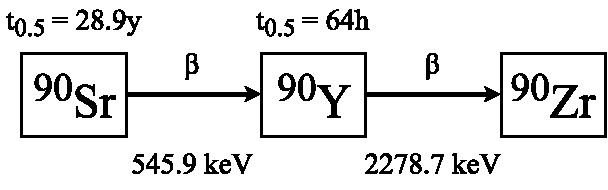
\includegraphics[width=7.5cm]{chain}
\caption{Decay chain for strontium-90 showing Q-values\cite{Qval} and half-lives\cite{half}}
\label{fig:chain}
\end{center}
\end{figure}

For example, when strontium-90 decays it first decays forming unstable yttrium-90 emitting $\beta$ particles with a Q-value (amount of energy released) of 545.9 keV\cite{Qval}. 
The unstable yttrium-90 then decays forming stable zirconium-90 emitting $\beta$ particles with a Q-value of 2278.7 keV\cite{Qval}.
This process is shown in Figure \ref{fig:chain}.
One should expect the $\beta$ particles from the yttrium to be able to penetrate further into a particular material than the $\beta$ particles from the strontium as their energy is greater.

In this experiment I investigated the presence of background radiation, dead time, if the count rate depends on the inverse square of the distance from the radioactive source and how the absorption of $\beta$ particles varies with the thickness of aluminium.

The overall aim of this experiment was to become familiar with sealed radioactive sources and Geiger counters and to become familiar with simple counting experiments and uncertainties due to Poisson distribution.

Figure \ref{fig:rail} is the experimental setup I used throughout.

\begin{figure}[!h]
\begin{center}
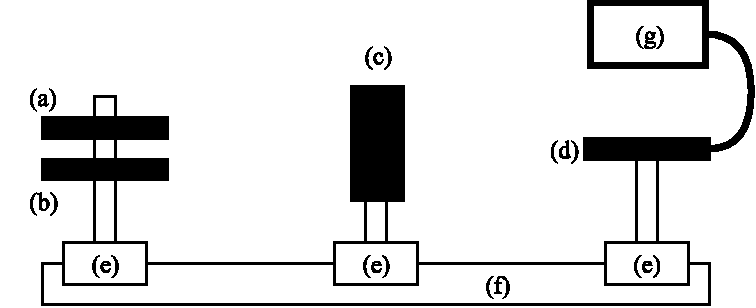
\includegraphics[width=7.5cm]{rail}
\caption{Diagram of experimental setup. (a) Source A; (b) source B; (c) slide holder; (d) GM tube; (e) holder; (f) optical rail and (g) counter. Each holder can be moved along the optical rail and clamped in position, and both source A and B can be removed or clamped into the holder. The slide holder is capable of holding many square-shaped slides at once. A stopwatch and measuring tape are also used along with this apparatus. Source A and B are both strontium-90.}
\label{fig:rail}
\end{center}
\end{figure}

When taking measurements it is important to consider the dead time and the background radiation.
Dead time is the period of time in which a detector is unable to record a pulse or a particle after it has already detected one.

\vspace{-3ex}

\begin{equation}
N=\dfrac{N_{1}-N_{0}}{1-\left(N_{1}-N_{0}\right)t_{d}}
\label{eq:true}
\end{equation}

Equation \ref{eq:true} is used to calculate the true count rate, $N$. $N_{0}$ is the background count rate; $N_{1}$ is the measured count rate and $t_{d}$ is the dead time.\cite{dead}

As radioactive decay follows a Poisson distribution the uncertainty in the number of counts, $N$ is $\sqrt{N}$.\cite{poisson} The fractional uncertainty is therefore $\dfrac{\sqrt{N}}{N}$ or simply $\dfrac{1}{\sqrt{N}}$.
The fractional uncertainty decreases as the number of counts increases. The count rate can be generalised as,

\vspace{-3ex}

\begin{equation}
\dfrac{N}{T} \pm \dfrac{\sqrt{N}}{T}\ s^{-1}
\label{eq:unc}
\end{equation}

\vspace{-3ex}

\vspace{-3ex}
\section{Background Radiation} 

\vspace{-2ex}
\subsection{Procedure}
\vspace{-3ex}

As I conducted this experiment in a lab where there were other radioactivity experiments happening I placed the GM tube far from other sources to minimise the radiation from these.
I removed both sources from the apparatus shown in Figure \ref{fig:rail}.
After turning on the GM tube and counter I simultaneously started the counter and stopwatch and let them run for 10 minutes.

After 10 minutes had elapsed I stopped the counter and recorded the number of counts in this period.

\vspace{-2ex}
\subsection{Results} 
\vspace{-3ex}

The number of counts, $N_{c}=302$. As this was recorded over a 10 minute period the count rate, 

\begin{center}
$N=\dfrac{N_{c}}{10\times60}=\dfrac{302}{600}=0.50\overline{3}\ s^{-1}$.
\end{center}

The fractional uncertainty according to Equation \ref{eq:unc} is 0.0559.
Therefore the percentage uncertainty is 5.59\%.

\vspace{-2ex}
\subsection{Discussion} 
\vspace{-3ex}

The background count rate is quite small although it still might be large enough to affect an experiment therefore it must be taken into consideration.
A percentage uncertainty closer to 1\% would have been ideal but as the count rate is so low it would have been impractical to wait long enough for it to be this low so I compromised and measured for 10 minutes.

\vspace{-3ex}
\section{Dead Time}

\vspace{-2ex}
\subsection{Procedure}
\vspace{-3ex}

I removed the slide holder from the apparatus shown in Figure \ref{fig:rail} and ensured that only source A was clamped in position 20 cm away from the GM tube.
I started the stopwatch and counter simultaneously and let them run for 60 seconds before stopping them to record the count and elapsed time.

I repeated the procedure above twice first inserting source B as well as source A and then removing source A such that there was only source B.

As count rate is proportional to the inverse square of distance\cite{inv} I took care not to move the other source when I was adding or removing one.
I took the measurements in the order A $\rightarrow$ A \& B $\rightarrow$ B so that I would only need to add and remove source A and B once.
If either were moved error would have been added to the measurements.

The measurements taken are shown in Table \ref{table:dead}.

\begin{table}[!h]
\centering
\begin{tabular}{|r|l|l|l|}
\hline
                        & $n_{A}$  & $n_{AB}$  & $n_{B}$ \\ \hline
Count               & 6374       & 13734       & 7911      \\ \hline
\% uncertainty  & 1.25\%   & 0.853\%    & 1.12\%   \\ \hline
\end{tabular}
\caption{Table of counts, n and their associated uncertainties from sources A and B.}
\label{table:dead}
\end{table}

\vspace{-3ex}

\subsection{Analysis} 
\vspace{-3ex}

I substituted Equation \ref{eq:true} into $N_{AB}=N_{A}+N_{B}$ but I let the background be zero as I was only interested in the measured count rate.
I then solved for the dead time, $t_{d}$ giving Equation \ref{eq:dead2}.

\vspace{-3ex}

\begin{equation}
t_{d}=\dfrac{1}{n_{AB}}\Bigg[1\pm\sqrt{1-\dfrac{n_{AB}}{n_{A}n_{B}}(n_{A}+n_{B}-n_{AB})}\Bigg]
\label{eq:dead2}
\end{equation}

I therefore found $t_{d}=1.40\times10^{-4}$ seconds with an uncertainty of $2.07\times10^{-6}$ seconds and a percentage uncertainty of 1.48\%.

I am pleased with the accuracy of this measurement of dead time as the percentage uncertainty is quite small.

\vspace{-3ex}
\section{Count Rate and Inverse Square of Distance} 
\vspace{-3ex}

The count rate should be proportional to the inverse square of the distance from the source.
This should only apply when the source is a point source.\cite{inv}

\vspace{-4ex}
\subsection{Procedure}
\vspace{-3ex}

Remove the slide holder from the apparatus shown in Figure \ref{fig:rail}.
With only one strontium-90 source in the holder move the holder close to the GM tube and measure the distance accurately with a tape measure.
Simultaneously start the stopwatch and counter.
Keep running the counter until there is a high enough number of counts for the uncertainty to be low.
I compromised between a large enough count and short enough time.
I recorded the count, elapsed time, and distance on a table.
I then increased the distance and repeated the measurements to get more data.
I did this 15 times, making sure that I took more measurements closer to the source and fewer further away.

To analyse the results I used \textit{Mathematica\textregistered} however \textit{Excel\textregistered} could be used instead.
I used Equation \ref{eq:true} to correct each of the count rates.
I then used Equation \ref{eq:unc} to find the uncertainty in the count rate.

After this I plotted a linearised log-log graph (Figure \ref{fig:dep}) of count rate and distance from GM tube.
I used a log-log graph to spread out the data points more evenly.

\vspace{-5ex}
\subsection{Results}
\vspace{-3ex} 

When I first graphed my data I noticed two anomalous results when the distance was 5 mm and 15 mm.
I removed these results from the graph.

\begin{figure}[!h]
\begin{center}
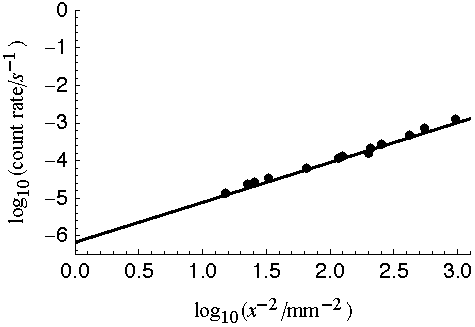
\includegraphics[width=7.5cm]{dep}
\caption{Linearised log-log graph of count rate and distance from GM tube}
\label{fig:dep}
\end{center}
\end{figure}

From Figure \ref{fig:dep}, the y-intercept is very close to zero when you take into account the effect of the log-log graph. 
I calculated the correlation to be 0.995095, suggesting a strong positive correlation.

\vspace{-5ex}
\subsection{Discussion}
\vspace{-3ex} 

As there is a strong positive correlation between count rate and distance$^{-2}$ and the y-intercept is very close to zero I can conclude that there is strong evidence that count rate is proportional to the inverse square of the distance from the source.
The two anomalous results occurred because at such a short distance the source is not a point source and does not obey the inverse square law.

\vspace{-5ex}
\section{Absorption by Aluminium} 
\vspace{-3ex}

When $\beta$ particles pass through matter they lose energy. 
The intensity of the radiation at a certain distance into a particular material is expressed by Equation \ref{eq:ix} where $I$ is the intensity at a distance $x$ into the material of absorption coefficient, $\mu$ for a particular energy of $\beta$ particles.
$I_{1}$ and $I_{2}$ are the intensities just before the material.\cite{abs} 
As strontium-90 has two different energies of $\beta$ particles in its decay chain Equation \ref{eq:ix} is a linear superposition of the intensity of the two different energies of $\beta$ particles.

\vspace{-3ex}

\begin{equation}
I\left( x\right) =I_{1}e^{-\mu_{1} x}+I_{2}e^{-\mu_{2} x}
\label{eq:ix}
\end{equation}

I verified this relationship in this part of the experiment.
(Intensity is analogous to the count rate.)

\vspace{-4ex}
\subsection{Procedure}
\vspace{-3ex}

As I completed this part of the experiment at a different time I calculated the background count rate again.
I set up the apparatus shown in Figure \ref{fig:rail} such that there was a slide holder and only one source.
I placed the source a distance from the GM tube where the count rate was {\raise.17ex\hbox{$\scriptstyle\mathtt{\sim}$}}500 s$^{-1}$ and then clamped everything in place.

I found the count rate at various thicknesses of aluminium. 
I took 6 measurements between 0 mm and 0.1 mm and I took 10 measurements between 0.1 mm and 1 mm.
I used thin slides that were labelled with their thickness.
I also used thicker slides. For these I used electronic vernier callipers to determine their thickness to an uncertainty of 0.005mm.

I placed slides in the slide holder to produce the desired thickness.
I started the counter and stopwatch simultaneously and let them run for 20 seconds before stopping them.
Using \textit{Excel\textregistered} I calculated the count rate of each by dividing the count by the elapsed time.
I used Equation \ref{eq:true} to correct each of the count rates.
Then I used Equation \ref{eq:unc} to find the uncertainty in the count rate.

I then plotted a linearised graph of count rate and thickness of aluminium as shown in Figure \ref{fig:al}.
Next I separated the two energies.
I used the data after the change of gradient to plot a linearised graph of the absorption of high energy $\beta$ particles and distance as there are no low energy particles in that region.
I used the data before it to plot a similar graph for the low energy particles but subtracted the count rate of the high energy particles at that point using the count rate and $\mu$ calculated from the high energy graph.
This step can be summarised by: $N_{low}(x)=N_{total}(x)-N_{0,high}e^{-\mu_{high} x}$.

\vspace{-2ex}
\subsection{Results} 
\vspace{-4ex}

\begin{figure}[!h]
\begin{center}
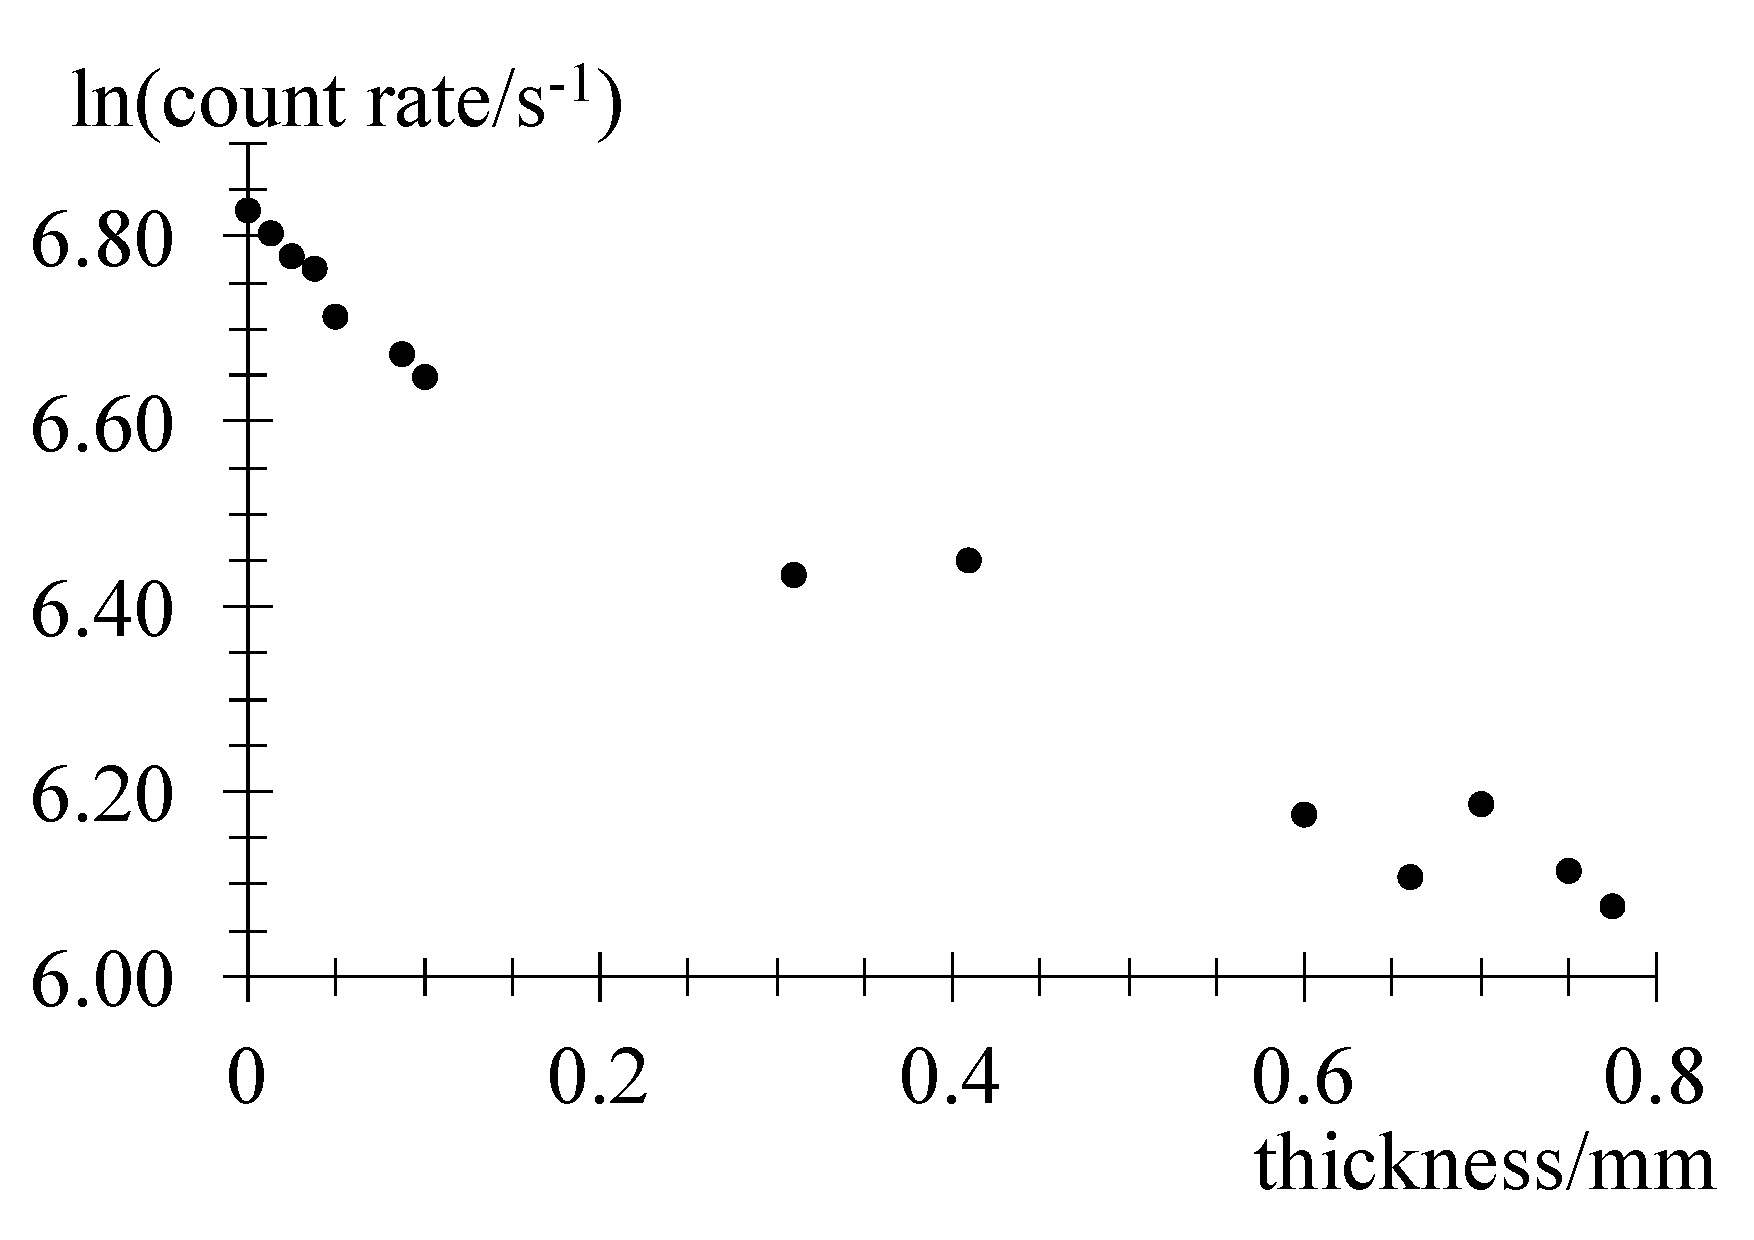
\includegraphics[width=7.5cm]{al}
\caption{Linearised graph of count rate and thickness of aluminium}
\label{fig:al}
\end{center}
\end{figure}

It can be seen in Figure \ref{fig:al} that between 0 mm and 0.3 mm the natural logarithm of the count rate decreases more quickly as thickness increases than between thicknesses of 0.3 mm and 0.8 mm.

From the linear graph for each energy of $\beta$ particle I found gradients, y-intercepts and correlations.
$\mu$ from Equation \ref{eq:ix} can be found by finding the negative of the gradient. 
$I_{1}$ and $I_{2}$ can be found by finding the inverse natural logarithm of the y-intercept.
These results are shown in Table \ref{table:ix}.

\vspace{0ex}

\begin{table}[!h]
\centering
\begin{tabular}{|r|l|l|}
\hline
\multicolumn{1}{|l|}{} & {High energy $\beta$} & {Low energy $\beta$} \\ \hline
{Gradient}            & {-0.8396}                       & {-26.952}                      \\
{$\mu$ / mm}       & {0.8396}                        & {26.952}                       \\ \hline
{y-intercept}         & {6.7248}                        & {4.7253}                       \\
{Count rate / s}    & {832.81}                        & {112.76}                       \\ \hline
{Correlation}    & {0.90061}                        & {0.90694}                       \\ \hline
\end{tabular}
\caption{Table of absorption coefficients, count rates and correlations for different energies of $\beta$ particles.}
\label{table:ix}
\end{table}

\vspace{-2ex}
\subsection{Discussion} 
\vspace{-3ex}

Some of the background radiation would have been absorbed by the aluminium hence affecting the background count rate.
Measuring the background each time would have introduced more error than the background itself as the source would have to be moved.
I therefore assumed that the change in background was negligible as the value was already very low.

As the absorption coefficient, $\mu$ is greater for low energy $\beta$ particles they get absorbed sooner. 
By 0.3 mm depth all of them have been absorbed.
From Figure \ref{fig:al} one can clearly see that after 0.3 mm the gradient changes.

As there was a strong positive correlation between the natural logarithm of the count rate and thickness of aluminium for each energy of $\beta$ particles the relationship described by Equation \ref{eq:ix} holds.

														\begin{comment}

\vspace{-3ex}
\section{Half-life of Barium-137m}
\vspace{-3ex} 

\vspace{-2ex}
\subsection{Procedure}
\vspace{-3ex}

\vspace{-2ex}
\subsection{Results} 
\vspace{-3ex}

\begin{figure}[!h]
\begin{center}
\includegraphics[width=7.5cm]{ba}
\caption{Graph of count rate and time with gridlines showing an estimation of the half-life of Ba-137m}
\label{fig:ba}
\end{center}
\end{figure}

\vspace{-2ex}
\subsection{Discussion} 
\vspace{-3ex}

														\end{comment}

\vspace{-4ex}
\section{Conclusion}
\vspace{-3ex} 

In the future I would like to explore more into the actual effect of background count rate and dead time instead of just measuring them and taking them into account in calculations.
I would recommend the use of a stopwatch that directly controls the counter as I found it difficult to turn them off or on simultaneously.

I succeeded in better understanding radioactive sources and how to measure counts with a Geiger counter.
I also explored some of the uncertainties arising as a result of the Poisson distribution.
I measured the background count rate and also the dead time.
It was verified that the count rate is proportional to the inverse square of the distance and that beta particles get absorbed by aluminium according to Equation \ref{eq:ix} ($I(x)=I_{0}e^{-\mu x}$).

\begin{thebibliography}{99}

\bibitem{gen} D. Halliday, R. Resnick, and J. Walker, {\it Fundamentals of Physics Extended}, 9th ed. (Wiley, 2003), pp. 1174--1181.
\bibitem{Qval} G. Audi {\it et al}, Chinese Physics C {\bf 36}, 1287 (2012).
\bibitem{half} NNDC,\ BNL,\ "Chart of Nuclides".\ [Online].\ Available:\ http://www.nndc.bnl.gov/chart/.\ [Accessed:\ 16/03/2016].
\bibitem{dead} Adapted from, A. Patil, PhD in Nuclear Engineering Thesis, Missouri University of Science and Technology, 2010.
\bibitem{poisson} S. E. Shnoll {\it et al}, Physics-Uspekhi {\bf 41}, 1025 (1998).
\bibitem{inv} T. Whyntie and B. Parker, Phy. Educ. {\bf 48}, 344 (2013).
\bibitem{abs} O. G\"{u}rler \& S. Yal\c{c}\i{}n, Ann. Nucl. Energy {\bf 32}, 1918 (2005).

\end{thebibliography} 

\end{document}